\documentclass[11pt, oneside]{article}   	% use "amsart" instead of "article" for AMSLaTeX format
\usepackage{geometry}                		% See geometry.pdf to learn the layout options. There are lots.
\geometry{letterpaper}                   		% ... or a4paper or a5paper or ... 
%\geometry{landscape}                		% Activate for for rotated page geometry
%\usepackage[parfill]{parskip}    		% Activate to begin paragraphs with an empty line rather than an indent
\usepackage{graphicx}				% Use pdf, png, jpg, or eps§ with pdflatex; use eps in DVI mode
								% TeX will automatically convert eps --> pdf in pdflatex		
\usepackage{amssymb}
\usepackage{amsmath}
\usepackage{parskip}
\usepackage{color}
\usepackage{hyperref}

\title{Analysis:  definitions}
%\author{The Author}
%\section{}
%\subsection*{}
\date{}							% Activate to display a given date or no date

\graphicspath{{/Users/telliott_admin/Dropbox/Tex/png/}}
% \begin{center} 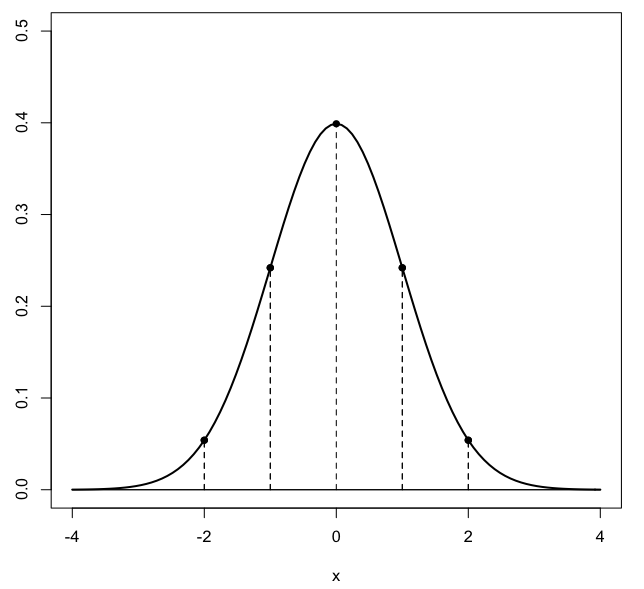
\includegraphics [scale=0.4] {gauss3.png} \end{center}
\begin{document}
\maketitle
\Large

$\bullet$  The set $X$ is \emph{bounded above} $\iff \exists \ M \in \mathbb{R} \ | \ \forall \ x \in X, x \le M$.

A closely related definition is the following:

$\bullet$  A function $f: X \rightarrow \mathbb{R}$ is \emph{bounded above} on X $\iff \exists \ M \in \mathbb{R} \ | \ \forall \ x \in X, x \le M$.

As an example $f(x) = x^2$ is \emph{not bounded above}.  The reason is that reading the definition, we must pick $M$ first.  Given $M$, we can always find a value of $x$ so that $f(x) > M$.

If we were allowed to pick $x$ first, then of course we could always find $M$ such that $f(x)  \le M$.  But that is not how the game is played.

\begin{center} 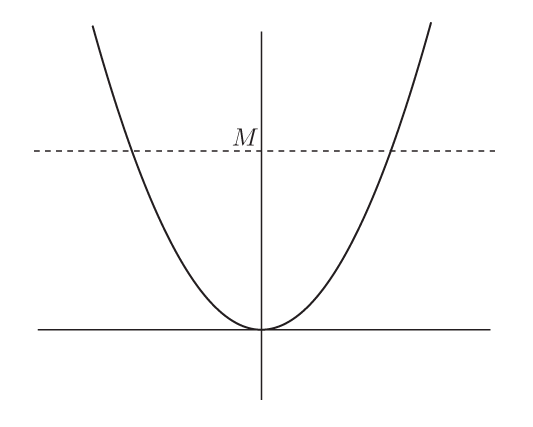
\includegraphics [scale=0.4] {x^2_not_bounded.png} \end{center}

\end{document}